\TieudeT{PHONG TỎA VẬT LÍ 12 - VẬT LÍ NHIỆT}
\subsubsection*{PHẦN I. Thí sinh trả lời câu hỏi từ câu 1 đến câu 18. Mỗi câu hỏi thí sinh chỉ chọn một phương án}
\setcounter{ex}{0}
\begin{ex}%Câu 15
	Chuyển động nào sau đây \textbf{không} được coi là chuyển động Brown?
	\choice
	{Chuyển động của các hạt bụi lơ lửng trong không khí khi quan sát dưới ánh nắng mặt trời vào buổi sáng}
	{Chuyển động của hạt phấn hoa trong nước}
	{Chuyển động của các hạt mực khi nhỏ các giọt mực vào nước}
	{\True Chuyển động thành dòng của các hạt bụi nhỏ trong ống khơi của nhà máy xi măng đang vận hành}
	\loigiai{}
\end{ex}
\begin{ex}%Câu 17
	\immini[thm]{Hình bên là đồ thị phác họa sự thay đổi nhiệt độ theo thời gian trong quá trình chuyển thể từ rắn sang lỏng của chất rắn kết tinh và của chất rắn vô định hình tương ứng là
		\choice[1]
		{đường (3) và đường (1)}
		{\True đường (3) và đường (2)}
		{đường (1) và đường (2)}
		{đường (2) và đường (3)}}
	{\begin{tikzpicture}[scale=.8,line width=1.5,>=stealth']
			\tkzDefPoints{0/-0.5/o, 5/-0.5/x, 0/5/y}
			\tkzDrawSegments[->,line width=1.5](o,x o,y)
			\tkzLabelPoint[below left](o){$O$}
			\tkzLabelPoint[below](x){Thời gian}
			\tkzLabelPoint[right](y){Nhiệt độ}
			\draw[thin,dashed] (0,2.5) -- (4,2.5);
			\draw[dotted,blue] (0.9,0.6) .. controls (3,1.5) and (2.5,3.5) .. (4.6,4.5);
			\draw[dashed,green] (0.9,0.6)node[below,black]{Rắn} --(3.5,0.6) --(3.5,3) --(4.6,4.5)node[above,black]{Lỏng};
			\draw[red] (1.5,2.5) -- (3.9,2.5);
			\draw [red] plot[smooth, tension=.7] coordinates {(0.9,0.6) (1,1.6) (1.1,2.1) (1.3121,2.4202) (1.5,2.5)};
			\draw[red]  plot[smooth, tension=.7] coordinates {(4.6,4.5) (4.5,3.6) (4.35,2.85) (4.15,2.55) (3.9,2.5)};
			\node[left] at (0,2.5) {$t_C$};
			\node[right] at (3.5,1.5) {$(1)$};
			\node[left] at (3.5,4) {$(2)$};
			\node[right] at (4.5,3) {$(3)$};
	\end{tikzpicture}}
	\loigiai{}
\end{ex}
\begin{ex}
	Khi sắp xếp độ lớn lực tương tác giữa các phân tử chất rắn, chất lỏng và chất khí theo thứ tự từ nhỏ đến lớn, cách sắp xếp nào sau đây là đúng?
	\choice
	{Khí, rắn, lỏng}
	{Rắn, khí, lỏng}
	{\True Khí, lỏng, rắn}
	{Rắn, lỏng, khí}
	\loigiai{}
\end{ex}
\begin{ex}
	Vào buổi sáng, sương trên lá hóa hơi thành hơi nước dưới ánh nắng mặt trời. Trong quá trình này, giữa các phân tử nước có
	\choice
	{\True lực hút và lực đẩy phân tử đều yếu đi}
	{lực hút phân tử mạnh lên còn lực đẩy phân tử yếu đi}
	{lực hút và lực đẩy phân tử đều mạnh lên}
	{lực hút phân tử yếu đi còn lực đẩy phân tử mạnh lên}
	\loigiai{}
\end{ex}
\begin{ex}
	Một thang đo nhiệt độ $X$ lấy nhiệt độ của nước tinh khiết đóng băng ở điều kiện chuẩn là $-10\ X$, lấy điểm sôi của nước tinh khiết ở áp suất chuẩn là $90\ X$. Nếu nhiệt độ của một vật đọc được trên nhiệt kế Celsius là $55^\circ C$ thì trên nhiệt kế $X$ có nhiệt độ bằng
	\choice
	{$30\ X$}
	{$55\ X$}
	{$40\ X$}
	{\True $45\ X$}
	\loigiai{}
\end{ex}
\begin{ex}
	Một số chất ở thể rắn như iodine (i-ốt), băng phiến, đá khô $(CO_2)$ ở thể rắn,.. có thể chuyển trực tiếp sang..(1).. khi nó..(2).. Hiện tượng trên gọi là sự thăng hoa. Ngược lại, với sự thăng hoa là sự ngưng kết. Điền cụm từ thích hợp vào chỗ trống.
	\choice
	{(1) thể lỏng; (2) toả nhiệt}
	{(1) thể hơi; (2) toả nhiệt}
	{(1) thể lỏng; (2) nhận nhiệt}
	{\True (1) thể hơi; (2) nhận nhiệt}
	\loigiai{}
\end{ex}
\begin{ex}
	Cho biết nước đá có nhiệt nóng chảy riêng là $\lambda = 3,4 . 10^5\  J/kg$ và nhiệt dung riêng $c = 2,09 . 10^3\  J/kg$. Nhiệt lượng cần cung cấp để làm nóng chảy hoàn toàn cục nước đá khối lượng 50 g và ở nhiệt độ $-20^{\circ} C$ có giá trị bằng
	\choice
	{190 kJ}
	{36 kJ}
	{\True 19 kJ}
	{1,9 kJ}
	\loigiai{}
\end{ex}
\begin{ex}
	Hình bên mô tả chuyển động phân tử ở các thể khác nhau. Hình cầu là phân tử, mũi tên là hướng chuyển động của phân tử. Thứ tự hình mô tả chuyển động phân tử tương ứng với thể khí, thể lỏng và thể rắn lần lượt là
	\begin{center}
		\begin{tikzpicture}[draw=Mapcolor, very thick, line join = round, line cap=round,>=stealth,font=\footnotesize,scale=1,line width=0.8]
			\draw (3.1,0) rectangle +(1.5,2); \path (3.1,0) -- +(1.5,0) node [pos=0.5,below]{a)};
			\draw[black] (3.5,1.5) circle(0.15);
			\draw[densely dotted] (4.2,1) circle(0.15) (3.4,0.35) circle(0.15);
			\draw[densely dotted,->](3.5,1.5) -- (4.2,1) ;
			\draw[densely dotted,->] (4.2,1) --(3.4,0.35);
			\draw[densely dotted,->] (3.4,0.35)--+(0.75,0);
		\end{tikzpicture}\hspace{1.5cm}
		\begin{tikzpicture}[draw=Mapcolor, very thick, line join = round, line cap=round,>=stealth,font=\footnotesize,scale=1,line width=0.8]
			\draw (3.1,0) rectangle +(1.5,2); \path (3.1,0) -- +(1.5,0) node [pos=0.5,below]{b)};
			\draw[black] (3.8,1) circle(0.15);
			\foreach \g in {0,45,90,135,180,225,270,315}{
				\path (3.8,1) coordinate (A)
				++(\g:0.15) coordinate (B)
				++(\g:0.3) coordinate (C);
				\draw[densely dotted,->](B) -- (C) ;};
		\end{tikzpicture}\hspace{1.5cm}
		\begin{tikzpicture}[draw=Mapcolor, very thick, line join = round, line cap=round,>=stealth,font=\footnotesize,scale=1,line width=0.8]
			\draw (3.1,0) rectangle +(1.5,2); \path (3.1,0) -- +(1.5,0) node [pos=0.5,below]{c)};
			\draw[black] (3.6,1.5) circle(0.15);
			\foreach \g in {0,45,90,135,180,225,270,315}{
				\path (3.6,1.5) coordinate (A)
				++(\g:0.15) coordinate (B)
				++(\g:0.3) coordinate (C);
				\draw[densely dotted,->](B) -- (C) ;};
			\draw[black] (4.1,0.55) circle(0.15);
			\foreach \g in {0,45,90,135,180,225,270,315}{
				\path (4.1,0.55) coordinate (A)
				++(\g:0.15) coordinate (B)
				++(\g:0.3) coordinate (C);
				\draw[densely dotted,->](B) -- (C) ;};
			\path (3.6,1.5)++(0:0.15) coordinate (M)
			(4.1,0.55) ++(90:0.15) coordinate (N);
			\draw[densely dotted,->](M) .. controls (4.4,1.3) .. (N);
		\end{tikzpicture}
	\end{center}
	\choice
	{\True a), c), b)}
	{a), b), c)}
	{c), b), a)}
	{b), a), c)}
	\loigiai{}
\end{ex}
\begin{ex}
	Phát biểu nào sau đây là đúng khi nói về sự đông đặc của một chất?
	\choice
	{\True Tỏa nhiệt ra môi trường}
	{Cần cung cấp nhiệt lượng}
	{Xảy ra ở cùng nhiệt độ với sự hóa hơi}
	{Xảy ra ở $0^{\circ} C$}
	\loigiai{}
\end{ex}
\begin{ex}%Câu 1
	Hiện tượng nào sau đây \textbf{không} liên quan đến sự nóng chảy?
	\choice
	{Cầu chì bị đứt khi dòng điện qua nó có cường độ lớn hơn giá trị cho phép}
	{Thép được nấu trong lò luyện kim}
	{\True Giọt nước đọng bên ngoài cốc nước đá}
	{Đá trong cốc nước chanh đá ngày càng nhỏ đi}
	\loigiai{}
\end{ex}
\begin{ex}%Câu 2
	Phân tích các tình huống sau, xem xét quá trình truyền nhiệt liên quan đến từng tình huống đó:
	\begin{itemize}
		\item[I. ]Rau nóng lên khi cho vào chảo nước sôi.
		\item[II. ] Ngăn đông nằm ở phía trên tủ lạnh, làm mát toàn bộ bên trong tủ lạnh.
		\item[III. ]Các thành phần điện tử của thiết bị vận hành trên trạm vũ trụ truyền nhiệt vào không gian.
	\end{itemize}
	Các tình huống I, II và III lần lượt tương ứng với các quá trình
	\choice
	{dẫn nhiệt, đối lưu và dẫn nhiệt}
	{đối lưu, bức xạ và đối lưu}
	{\True dẫn nhiệt, đối lưu và bức xạ}
	{bức xạ, dẫn nhiệt và bức xạ}
	\loigiai{}
\end{ex}
\begin{ex}
	Người ta dùng một ấm điện bằng nhôm có khối lượng $m_1=0,4\ kg$ để đun sôi một lượng nước $m_2=3\ kg$ thì sau $25$ phút nước sẽ sôi (biết nhiệt độ sôi của nước ở áp suất tiêu chuẩn là $100^{\circ} C$). Bếp điện có hiệu suất $H=80 \%$ và được dùng ở mạng điện xoay chiều có hiệu điện thế hiệu dụng $U=220\ V$. Nhiệt độ ban đầu của ấm nước là $20^{\circ} C$, nhiệt dung riêng của nhôm là $c_1=920\ J/(kg.K)$; nhiệt dung riêng của nước là $c_2=4,18\ kJ /(kg.K)$. Cường độ cực đại dòng điện chạy qua bếp điện có giá trị xấp xỉ bằng
	\choice
	{$3,91\ A$}
	{$3,13\ A$}
	{\True $5,53\ A$}
	{$2,50\ A$}
	\loigiai{}
\end{ex}
\begin{ex}%Câu 1
	Nội dung nào dưới đây \textbf{không} thể hiện sự bay hơi của vật chất?
	\choice
	{Bật quạt sau khi lau sàn nhà}
	{\True Xuất hiện các giọt nước ở thành ngoài cốc nước giải khát có đá khi để trong không khí}
	{Sử dụng khí gas $(R-32)$ trong các thiết bị làm lạnh của máy điều hoà không khí}
	{Sản xuất muối của các diêm dân}
	\loigiai{}
\end{ex}
\begin{ex}%Câu 4
	Trường hợp nào dưới đây làm biến đổi nội năng của vật \textbf{không phải} do thực hiện công?
	\choice
	{Khuấy nước}
	{Mài dao}
	{\True Nung đồng trong lò}
	{Đóng đinh}
	\loigiai{}
\end{ex}
\begin{ex}%Câu 13
	Một thước cm được đặt dọc theo một nhiệt kế thủy ngân chưa được chia vạch như hình dưới đây. Trên nhiệt kế chỉ đánh dấu điểm đóng băng và điểm sôi của nước tinh khiết ở áp suất tiêu chuẩn. Giá trị nhiệt độ đang hiển thị trên nhiệt kế là
	\begin{center}
		\begin{tikzpicture}[rotate = 0, scale = 0.75,draw=Mapcolor, very thick,  >=stealth]
			\draw[thick, line width = 1,rounded corners=4pt](-0.5,0) rectangle (12,0.4);
			\fill[black,thick, line width = 1,rounded corners=3pt](-0.45,0.05) rectangle (0.3,0.35);
			\draw[thick, line width = 0.8,rounded corners=2pt](-0.3,0.12) rectangle (11.8,0.28);
			\fill[black,thick, line width = 1,rounded corners=1pt](-0.3,0.12) rectangle (6.6,0.28);
			\draw[thick, line width = 1](-1,-1) rectangle (12.5,0);
			\draw (-0.5,-0.25) node []{cm};
			\foreach \i in {0,...,60}\draw (0.2*\i,-0.1)--++(0,-0.2);
			\foreach \i in {0,...,12}\draw (1*\i,-0.1)--++(0,-0.35);
			\foreach \i in {0,...,12}{\draw (\i,-0.7) node{\i};}
			\draw[-,dashed, line width = 1] (1,0) -- (1,0.6);
			\draw[-,dashed, line width = 1] (11,0) -- (11,0.6);
			\draw[-,dashed, line width = 1] (6.6,0.1) -- (6.6,-1.4) node [below]{6,6};
			\draw[-,thick, line width = 1] (1,0.6) -- (1.5,1) node [above]{Điểm đóng băng};
			\draw[-,thick, line width = 1] (11,0.6) -- (11.5,1) node [above]{Điểm sôi};
		\end{tikzpicture}
	\end{center}
	\choice
	{\True $56\ ^{\circ}C$}
	{$60\ ^{\circ}C$}
	{$66\ ^{\circ}C$}
	{$44\ ^{\circ}C$}
	\loigiai{}
\end{ex}
\begin{ex}
	Phát biểu nào sau đây là \textbf{sai} khi nói về sự nóng chảy và sự đông đặc?
	\choice
	{Các chất khác nhau sẽ nóng chảy (hay đông đặc) ở nhiệt độ khác nhau}
	{Đối với một chất nhất định, nếu nóng chảy ở nhiệt độ nào thì sẽ đông đặc ở nhiệt độ ấy}
	{\True Nhiệt độ của vật sẽ tăng dần trong quá trình nóng chảy và giảm dần trong quá trình đông đặc}
	{Phần lớn các chất nóng chảy (hay đông đặc) ở một nhiệt độ nhất định}
	\loigiai{}
\end{ex}
\begin{ex}
	Gọi $\rho_1, \rho_2, \rho_3$ và $\rho_4$ lần lượt là khối lượng riêng của các vật làm bằng thiếc, nhôm, sắt và niken. Biết $\rho_2 < \rho_1 < \rho_3 < \rho_4$. Coi như toàn bộ độ giảm cơ năng chuyển hết thành nội năng của vật. Nội năng của vật nào tăng nhanh nhất khi ta thả rơi bốn vật có cùng thể tích và cùng hình dạng từ cùng một độ cao xuống đất? 
	\choice
	{Vật bằng sắt}
	{Vật bằng thiếc}
	{\True Vật bằng niken}
	{Vật bằng nhôm}
	\loigiai{}
\end{ex}
\begin{ex}
	Thả vào $0,5\ kg$ nước ở nhiệt độ $t_1=20^{\circ} C$ một cục nước đá khối lượng $0,5\ kg$ và nhiệt độ $t_2$ $=-15^{\circ} C$. Cho biết nhiệt dung riêng của nước $c_1=4200\ J/kg.K$, của nước đá $c_2=2100\ J/kg.K$. Nhiệt nóng chảy riêng của nước đá $\lambda=3,4 . 10^5\ J/kg$. Nhiệt độ của hỗn hợp sau khi cân bằng nhiệt được thiết lập là
	\choice
	{$5^{\circ} C$}
	{$10^{\circ} C$}
	{\True $0^{\circ} C$}
	{$2^{\circ} C$}
	\loigiai{}
\end{ex}
\subsubsection*{PHẦN 2. Thí sinh trả lời từ câu 1 đến câu 4. Trong mỗi ý a), b), c), d) ở mỗi câu, thí sinh chọn đúng hoặc sai.}
\setcounter{ex}{0}
\begin{ex}
	Để đo nhiệt hóa hơi riêng của nước, cho các dụng cụ sau: Cân điện tử (1), biến thế nguồn (2), Oát kế có tích hợp chức năng đo thời gian (3), nhiệt lượng kế kèm dây điện trở (4), nhiệt kế điện tử (5) (hình bên).
	\begin{center}
		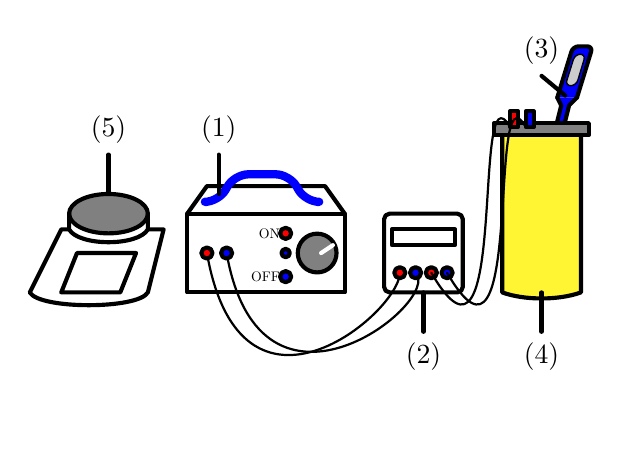
\begin{tikzpicture}[scale = 0.5, line join=round, line cap=round, >=stealth,line width=1.5]
			\begin{scope}[yshift= 0.75 cm]% Nhiệt kế
				\draw[rounded corners=2,fill=blue] (11.4,2.2) -- (11.8,3.5) -- (12.3,3.5) -- (11.9,2.2);
				\draw[rounded corners=2,fill=black!20,line width = 0.5] (11.6,2.5) -- (11.85,3.3) -- (12.12,3.3) -- (11.88,2.5) -- cycle;
				\draw[fill=blue] (11.9,2.2) -- (11.7,2) -- (11.2,0) --(11,0)-- (11.5,2)--(11.4,2.2);
			\end{scope}
			%\draw[fill=black] (0,0) circle (2pt);
			%\draw[dashed,line width=0.2] (-4,-4) grid (7,7);
			\draw[fill=gray](0,0) ellipse (1cm and 0.5cm);
			\draw (-1,0) -- (-1,-0.4) ..controls +(-60:0.5) and +(-120:0.5)..(1,-0.4) -- (1,0);
			\draw (-1,-0.4) -- (-1.2,-0.4) -- (-2,-2) ..controls +(-60:0.5) and +(-120:0.5).. (1,-2) -- (1.4,-0.4) -- (1,-0.4);
			\draw (-1.2,-2) -- (-0.8,-1) -- (0.7,-1) -- (0.3,-2) -- cycle;
			\draw (2,-2) rectangle (6,0);
			\draw (2,0) -- (2.5,0.7) -- (5.5,0.7) -- (6,0);
			\draw[rounded corners=2] (7,-2) rectangle (9,0);
			\draw (7.2,-0.8) rectangle (8.8,-0.4);
			\draw [line width=0.8](2.5,-1) .. controls +(-80:5) and +(-90:1) ..(7.4,-1.5);
			\draw [line width=0.8](3,-1) .. controls +(-80:5) and +(-45:1) ..(7.8,-1.5);
			\draw[fill=red] (2.5,-1) circle (4pt);
			\draw[fill=blue] (3,-1) circle (4pt);
			\draw[fill=red] (7.4,-1.5) circle (4pt);
			\draw[fill=blue] (7.8,-1.5) circle (4pt);
			\draw[fill=red] (8.2,-1.5) circle (4pt);
			\draw[fill=blue] (8.6,-1.5) circle (4pt);
			\draw[fill=gray] (5.3,-1) circle (14pt);
			\draw[white] (5.4,-1) -- (5.7,-0.8);
			\draw[fill=red] (4.5,-0.5) circle (4pt) node [scale = 0.5,left = 0.05]{ON} ;
			\draw[fill=blue] (4.5,-1.6) circle (4pt) node [scale = 0.5,left = 0.05]{OFF};
			\draw[fill=blue] (4.5,-1) circle (3pt);
			\draw[rounded corners=5,blue,line width=3] (2.5,0.3) -- (2.8,0.3) -- (3.2,1) -- (4.6,1) -- (5,0.3)-- (5.3,0.3);
			\draw[fill=yellow!80] (10,2) -- (10,-2) ..controls +(-20:0.6) and +(-160:0.6).. (12,-2)--(12,2);
			\draw[fill=gray] (9.8,2) rectangle (12.2,2.3);
			\draw[fill=red] (10.2,2.2) rectangle (10.4,2.6);
			\draw[fill=blue] (10.6,2.2) rectangle (10.8,2.6);
			\draw [line width=0.8] (8.2,-1.5) .. controls +(-60:4) and +(120:2).. (10.2,2.2);
			\draw [line width=0.8] (8.6,-1.5) .. controls +(-60:4) and +(120:2).. (10.6,2.2);
			\draw (0,0.5) -- (0,1.5) node [above] {(5)};
			\draw (2.8,0.5) -- (2.8,1.5) node [above] {(1)};
			\draw (8,-2) -- (8,-3) node [below] {(2)};
			\draw (11,-2) -- (11,-3) node [below] {(4)};
			\draw (11,3.5) node [above] {(3)} -- (11.6,3);
		\end{tikzpicture}
	\end{center}
	\choiceTFt
	{\True Có thể sử dụng các dụng cụ trên để đo nhiệt hóa hơi riêng của nước ở nhiệt độ $100^{\circ} C$}
	{\True Tiến hành thí nghiệm như sau: Đặt nhiệt lượng kế lên cân, đổ nước nóng vào nhiệt lượng kế sao cho toàn bộ dây điện trở chìm trong nước; Nối Oát kế với nhiệt lượng kể và mở nắp nhiệt lượng kế; Xác định khối lượng nước trong bình; Bật nguồn điện, đun sôi nước trong nhiệt lượng kế; Quan sát ghi số chỉ trên đồng hồ đo thời gian, Oát kế, cân vào bảng số liệu; Tắt nguồn}
	{Quan sát số chỉ trên cân, Oát kế, đồng hồ đo thời gian thu được bảng số liệu như bảng dưới.
		\begin{center}
			\begin{tabular}{|c|c|c|c|c|c|c|}\hline \begin{tabular}{c} Thời gian \\$\tau(s)$\end{tabular}&0&120&240&360&480&600 \\\hline \begin{tabular}{c} Công suất \\$P(W)$\end{tabular}&0&15,21&15,19&15,21&15,23&15,19 \\\hline \begin{tabular}{c} Khối lượng \\$m(kg)$\end{tabular}&0,1200&0,1191&0,1184&0,1179&0,1170&0,1161 \\\hline\end{tabular}
		\end{center}
		Từ số liệu trên, vẽ được đồ thị khối lượng $m(kg)$ theo thời gian $\tau(s)$ có dạng đường thẳng đi qua gốc tọa độ}
	{Từ số liệu trên, tính được nhiệt hóa hơi riêng của nước ở $100^{\circ} C$ là $2,23 . 10^6\ J / kg$}
\end{ex}
\begin{ex}%Câu 19
\immini[thm]{Trong thí nghiệm đo nhiệt hoá hơi riêng của nước sử dụng ấm đun có công suất $1200\ W$. Khi nước sôi, mở nắp ấm đun để nước bay hơi. Một bạn học sinh thu được khối lượng nước còn lại trong ấm $m(g)$ theo thời gian $t(s)$ kể từ lúc nước sôi và khối lượng nước trong bình là $m_0=350\ g$ như bảng sau đây. Biết hao phí nhiệt lượng là $1,5\%$.}
	{\begin{tabular}{|c|c|c|}
			\hline Lần đo&$m(g)$&$t(s)$ \\
			\hline 1&300&100 \\
			\hline 2&250&203 \\
			\hline 3&200&304 \\
			\hline 4&150&406 \\
			\hline 5&100&505 \\
			\hline
		\end{tabular}
	}
	\choiceTFt
	{Nhiệt hoá hơi riêng của một chất là nhiệt lượng cần để $1\ kg$ chất đó chuyển hoàn toàn từ thể lỏng sang thể khí ở nhiệt độ nóng chảy}
	{\True Trong hệ SI, đơn vị đo của nhiệt hoá hơi riêng là $J/kg$}
	{Giá trị trung bình nhiệt hoá hơi riêng của nước trong thí nghiệm này là $2389,216\ J/g$ (trong mỗi lần đo tính trực tiếp nhiệt hoá hơi riêng của nước theo giá trị thời gian $t$ cho trong bảng)}
	{Sai số tuyệt đối trung bình của phép đo trong thí nghiệm này là $10,8 \ J\ /g$}
\end{ex}
\begin{ex}%Câu 20
\impicinpar{Năng lượng mặt trời là một nguồn năng lượng thân thiện với môi trường, ngày nay để tiết kiệm điện và bảo vệ môi trường rất nhiều hộ gia đình đã sử dụng bình nước nóng năng lượng mặt trời. Hình bên là bình nước nóng năng lượng mặt trời, diện tích tấm hấp thụ năng lượng mặt trời là $2\ m^2$ và thể tích bình chứa $200$ lít nước ở nhiệt độ $25\ ^{\circ}C$. Giả sử cường độ sáng trung bình của mặt trời những ngày có nắng là $1370\ W/m^2$, chỉ $60\%$ năng lượng mặt trời được hấp thụ truyền cho nước trong bình và bỏ qua sự trao đổi nhiệt của bình với môi trường. Cho khối lượng riêng của nước là $1000\ kg/m^3$, nhiệt dung riêng của nước là  $(4200\ J/kg.K)$.}
	{\begin{tikzpicture}[scale = 0.65, line join=round, line cap=round, >=stealth,line width=1.5]
			\draw[line width=4,gray] (4.7,4.6) circle (1.3cm);
			\draw[top color=red, bottom color=blue!70] (4.7,4.6) circle (1.2cm);
			\draw[line cap=butt,line width=4] (5.7,0) -- (5.7,3.7) (0,0) -- (4.1,3.5) (0,0) -- (0.65,0.5) -- (5.7,0.5) (4,0.5)--(5.7,2) (3.7,3.16) -- (5.7,3.16);
			\draw[double=white,double distance=1mm,rounded corners=5] (4.1,3.7)--(0.4,0.5)--(0,1)--(3.8,4.2);
			\draw[blue,line width=4,line cap=butt] (5.6,4) -- (6.7,4) -- (6.7,1.6);
			\draw[->,blue] (7,1) node [below,align=center,black] {Đường\\nước vào}-- (7,2);
			\draw[->,red] (1.2,4.4) -- (2,3.6);
			\draw[->,red](0.6,3.8)node[above,rotate=42] {Bức xạ mặt trời} -- (1.4,3);
			\draw[->,red] (6.2,5) -- (7,5) node [above right,align=center,violet] {Đường \\nước ra};
			\draw[red,line width=4,line cap=butt] (5.4,4.7) -- (7,4.7);
			\foreach \x/\y in {3.5/3.45}{
				\draw[blue,->] (\x,\y) -- ({\x-0.5},{\y-0.45});
				\draw[blue,->,xshift=-1cm,yshift=-0.85cm] (\x,\y) -- ({\x-0.5},{\y-0.45});
				\draw[blue,->,xshift=-2cm,yshift=-1.7cm] (\x,\y) -- ({\x-0.5},{\y-0.45});
				\draw[red,<-] (\x,{\y+0.2}) -- ({\x-0.5},{\y-0.25});
				\draw[red,<-,xshift=-1cm,yshift=-0.85cm] (\x,{\y+0.2}) -- ({\x-0.5},{\y-0.25});
				\draw[red,<-,xshift=-2cm,yshift=-1.7cm] (\x,{\y+0.2}) -- ({\x-0.5},{\y-0.25});}
		\end{tikzpicture}
	}
	\choiceTFt
	{Trong bình nước nóng năng lượng mặt trời, quang năng được chuyển hóa thành điện năng}
	{\True Trong khoảng thời gian $2\ h$ có nắng nước trong bình đã nóng thêm gần đúng $14,1\ ^{\circ}C$}
	{Thời gian có nắng để lượng nước trong bình sôi là $8,5\ h$}
	{\True Biết giá tiền điện là $1800$ đồng/kWh, so với việc sử dụng bếp điện có hiệu suất $80\%$ để làm nước trong bình nóng đến $75\ ^{\circ}C$, dùng bình nước nóng năng lượng mặt trời đã tiết kiệm được số tiền điện là $26250$ đồng}
\end{ex}
\begin{ex}%Câu 21
Hình bên là đồ thị mô tả nhiệt độ tại một địa điểm ở vùng ôn đới vào một ngày mùa đông.
		\immini{\choiceTFt
		{\True Nhiệt độ trên được ghi nhận theo thang đo nhiệt độ Celsius}
		{Tại thời điểm $10\ h$, nhiệt độ ghi nhận theo thang đo nhiệt độ Kelvin là $278\ K$}
		{Độ chênh lệch nhiệt độ lớn nhất giưa các thời điểm trong ngày là $8\ ^{\circ}C$}
		{\True Nhiệt độ thấp nhất trong ngày ghi nhận theo thang đo nhiệt độ Kelvin là $263\ K$}}
	{\begin{tikzpicture}[scale = 0.5, line join=round, line cap=round, >=stealth]
			\draw[->] (0,0)--(13.5,0) node[below] {Thời điểm (h)};
			\draw[->] (0,-10.5)--(0,2.5) node[right] {Nhiệt độ $(^\circ C)$};
			% \draw[gray!100,dashed] (0,0) grid[xstep=1,ystep=1] (6.5,2.5);
			\foreach \x in {2,4,6,8,10,12}{\draw [fill = black] (\x/2,0) circle(2pt) node [above]{\x};};
			\foreach \x in {14,16}{\draw [fill = black] (\x/2,0) circle(2pt) node [below]{\x};};
			\foreach \x in {18,20,22,24}{\draw [fill = black] (\x/2,0) circle(2pt) node [above]{\x};};
			\foreach \x in {-10,-9,-8,-7,-6,-5,-4,-3,-2,-1,0,1,2}{\draw [fill = black] (0,\x) circle(2pt) node [left]{\x};};
			\draw[-,thick, line width = 1.5] (0,-7)-- (1,-8) circle(2pt)-- (2,-9) circle(2pt)  -- (3,-10) circle(2pt)-- (4,-8) circle(2pt) -- (5,-5) circle(2pt)-- (6,-1)circle(2pt) -- (7,2)circle(2pt)-- (8,1)circle(2pt) -- (9,0)circle(2pt) -- (10,-2)circle(2pt) -- (11,-3)circle(2pt) -- (12,-3)circle(2pt);
			\draw[-,dashed, line width = 0.5] (0,-10) -- (3,-10) -- (3,0);
			\draw[-,dashed, line width = 0.5] (0,-5) -- (5,-5) -- (5,0);
			\draw[-,dashed, line width = 0.5] (0,-1) -- (6,-1) -- (6,0);
			\draw[-,dashed, line width = 0.5] (0,2) -- (7,2) -- (7,0);
			\draw[-,dashed, line width = 0.5] (0,1) -- (8,1) -- (8,0);
			\draw[-,dashed, line width = 0.5] (0,-2) -- (10,-2) -- (10,0);
			\draw[-,dashed, line width = 0.5] (0,-3) -- (11,-3) -- (11,0);
			\draw[-,dashed, line width = 0.5] (0,-3) -- (12,-3) -- (12,0);
			\draw[-,dashed, line width = 0.5] (0,-8) -- (1,-8) -- (1,0);
			\draw[-,dashed, line width = 0.5] (0,-9) -- (2,-9) -- (2,0);
			\draw[-,dashed, line width = 0.5] (1,-8) -- (4,-8) -- (4,0);
		\end{tikzpicture}
	}
\end{ex}
\subsubsection*{PHẦN 3. Thí sinh trả lời từ câu 1 đến câu 6.}
\setcounter{ex}{0}
\begin{ex}
	Trong một thí nghiệm, người ta thả rợi không vận tốc ban đầu một viên bi thép từ độ cao $200\ m$ so với mặt đất, khi vừa chạm đất nó có tốc độ $144 \ km/h$. Cho biết nhiệt dung riêng của thép $c= 460 \ J/kg.K$ và lấy $g=9,8 \ m/s^2$. Viên bi thép đã nóng thêm bao nhiêu ${ }^{\circ} C$ khi vừa chạm đất, nếu cho rằng toàn bộ công cản của không khí chỉ dùng để làm nóng viên bi thép (làm tròn kết quả đến chữ số hàng phần trăm)?
	\shortans[oly]{2,52}
\end{ex}
\begin{ex}%Câu 23
\impicinpar{Một bàn ủi có thể hoạt động được với dòng điện một chiều và xoay chiều. Đế của bàn ủi có khối lượng $400\ g$ được làm từ hợp kim chịu nhiệt, nhiệt dung riêng của đế là $890\ J/kg$.K. Sơ đồ mạch điện của bàn ủi (hình bên) bao gồm các bộ phận: điện trở Shunt (1) có giá trị $8\ \Omega$, đèn báo hiệu (2) có điện trở $2\ \Omega$, cuộn dây điện trở (3) coi như điện trở thuần có giá trị điện trở $98,4\ \Omega$. Cắm bàn ủi vào mạng điện có hiệu điện thế $220\ V$. Biết nhiệt độ ban đầu của bàn ủi là $22\ ^{\circ}C$; $80\%$ nhiệt lượng tỏa ra trên dây điện trở (3) được dùng làm nóng đế bàn ủi và bàn ủi có thể là được quần áo khi nhiệt độ của đế đạt giá trị nhỏ nhất là $180\ ^{\circ}C$. Sau khoảng thời gian ngắn nhất là bao nhiêu giây kể từ lúc bắt đầu cắm điện thì bàn ủi có thể là được quần áo (làm tròn kết quả đến chữ số hàng đơn vị)?}
	{\begin{tikzpicture}[scale = 1, line join=round, line cap=round, >=stealth]
			\draw (0,0) to[european resistor = $1$] (0,3) ;
			\draw (0,0.5) -- (1.5,0.5) to [lamp = 2] (1.5,2.5) -- (0,2.5);
			% \draw [->, thick] (0.6,-0.6) -- (1.4,0.6);% Dấu biến trở 
			\draw[decoration={aspect=0.1, segment length=2mm, amplitude=2mm,coil},decorate] (0.5,0) -- (1.5,0);
			\draw[-,thick, line width = 1] (0,3) -- (2.5,3) -- (2.5,1.75) circle(2pt) ;
			\draw[-,thick, line width = 1] (0,0) -- (0.5,0);
			\draw[-,thick, line width = 1] (1.5,0) -- (2.5,0) -- (2.5,1.25) circle(2pt) ;
			\draw (1,-0.5) node []{3};
		\end{tikzpicture}
	}
	\shortans[oly]{148}
\end{ex}
\textit{\textbf{Sử dụng các thông tin sau cho Câu 3 và Câu 4:}} Vào một số thời điểm trong năm, người ta quan sát thấy sự gia tăng đáng kể về số lượng sao băng trên bầu trời. Hiện tượng này được gọi là mưa sao băng, trong đó nổi bật nhất là mưa sao băng Perseid và Leonid. Mưa sao băng xảy ra khi Trái Đất đi qua quỹ đạo của một sao chổi để lại đám mây hạt trên đường đi của nó. Hầu hết các hạt này đều nhỏ như hạt bụi và khi xâm nhập vào bầu khí quyển Trái Đất, chúng bị nung nóng do ma sát với không khí và tạo ra những vệt sáng mà chúng ta quan sát được.
\begin{ex}
	Một hạt đi vào bầu khí quyển Trái Đất và bị dừng lại hoàn toàn do lực ma sát với không khí sau khi đi được quãng đường $1,5\ km$. Bỏ qua công của trọng lực trong sự dịch chuyển này. Nếu động năng ban đầu của nó bằng $4,5.10^4\ J$ thì lực ma sát trung bình có độ lớn là bao nhiêu newton? 
	\SA[oly]{30}
\end{ex}
\begin{ex}
	Giả sử một hạt có khối lượng $0,1\ g$ khi đi vào khí quyển thì nhiệt độ của nó tăng lên $2400^{\circ}C$. Biết nhiệt dung riêng của vật liệu tạo nên hạt là $0,9\ J/(g.{}^{\circ} C)$. Nhiệt lượng cần thiết để tạo ra sự tăng nhiệt độ này là bao nhiêu J?
	\SA[oly]{216}
\end{ex}
\begin{ex}
	Người ta dùng một chùm tia laze $CO_2$ có công suất $10\ W$ làm dao mổ. Tia laze chiếu vào chỗ mổ sẽ làm nước ở phần mô chỗ đó bốc hơi và mô bị cắt. Nhiệt dung riêng của nước là $4186\  J/kg.K$. Nhiệt hóa hơi riêng của nước là $L=2260\  kJ/kg$, nhiệt độ cơ thể là $37^{\circ} C$, khối lượng riêng của nước $1000\  kg/m^3$. Biết chùm laze có bán kính là $r=0,1\  mm$ và di chuyển với vận tốc $0,5\  cm/s$ trên bề mặt mô mềm. Chiều sâu tối đa của vết mổ xấp xỉ bằng bao nhiêu mm (làm tròn kết quả đến chữ số hàng đơn vị)?
	\SA[oly]{4}
\end{ex}
\begin{ex}
	Người ta đặt một viên bi đặc bằng sắt bán kính $R=6\  cm$ đã được nung nóng tới nhiệt độ $t=325^{\circ} C$ lên một khối nước đá rất lớn ở $0^{\circ} C$. Bỏ qua sự dẫn nhiệt của nước đá và sự nóng lên của đá đã tan. Cho khối lượng riêng của sắt là $D=7800\  kg/m^3$, của nước đá là $D_0=915\  kg/m^3$. Nhiệt dung riêng của sắt là $460\  J/kg.K$, nhiệt nóng chảy riêng của nước đá là: $3,4.10^5\  J/kg$. Viên bi chui vào nước đá đến độ sâu là bao nhiêu cm (làm tròn kết quả đến chữ số hàng đơn vị)?
	\SA[oly]{32}
\end{ex}


